% !TeX root = surprises.tex

\chapter{A Compass Is Sufficient}\label{c.compass}

%%%%%%%%%%%%%%%%%%%%%%%%%%%%%%%%%%%%%%%%%%%%%%%%%%%%%%%%%%%%%%%

\abstract*{The Mohr-Mascheroni Theorem shows that any construction that can be carried out using a straightedge and compass can be carried out with only a compass.}

%%%%%%%%%%%%%%%%%%%%%%%%%%%%%%%%%%%%%%%%%%%%%%%%%%%%%%%%%%%%%%%

\index{Construction!compass@with only a compass|(}
In 1797 Lorenzo Mascheroni\index{Mascheroni, Lorenzo} proved that any construction carried out with a straightedge and compass can be carried out with only a compass. Later it came to light that this theorem had already been proved by Georg Mohr\index{Mohr, Georg} in 1672.\index{Mohr-Mascheroni theorem}
After explaining in Sect.~\ref{s.compass-what} what is meant by performing a construction with only a compass, the proof is presented in stages starting with four auxiliary constructions: reflection of a point (Sect.~\ref{s.reflection}), construction of a circle with a given radius (Sect.~\ref{s.circle}), addition and subtraction of line segments (Sect.~\ref{s.add-subtract}) and construction of a line segment as a ratio of segments (Sect.~\ref{s.three}). Section~\ref{s.two-lines} shows how to find the intersection of two lines and Sect.~\ref{s.line-circle} shows how to find the intersection of a line and a circle.

\section{What Is a Construction With Only a Compass?}\label{s.compass-what}

Figure~\ref{f.compass-equi} shows the construction of an equilateral triangle using a straightedge and compass. How can we construct a triangle without the line segments $\overline{AB}, \overline{AC}, \overline{BC}$? A line segment is defined by two points, so it is sufficient to construct these points in order to obtain a construction equivalent to the one with a straightedge (Fig.~\ref{f.compass-equi-only}). There is no need to actually \emph{see} the line segments.
There will be lines in the figures in this chapter, but they are used only to understand the construction and the proof of its correctness. It is important to convince yourself that the construction itself uses only a compass.
\begin{figure}[ht]
\subfigures
\leftfigure[c]{
\begin{tikzpicture}[scale=0.6]
\coordinate (A) at (0,0);
\coordinate (B) at (4,0);
\vertex{A};
\vertex{B};
\draw (A) node[below left] {$A$} -- (B) node[below right] {$B$};
\draw[name path=larc] (A) ++(-10:4cm) arc (-10:80:4cm);
\draw[name path=rarc] (B) ++(-170:4cm) arc (-170:-260:4cm);
\path [name intersections={of=larc and rarc,by={t}}];
\node[above right,xshift=-2pt,yshift=3pt] at (t) {$C$};
\vertex{t};
\draw (A) -- (t);
\draw (B) -- (t);
\end{tikzpicture}
}
\hfill
\rightfigure[c]{
\centering
\begin{tikzpicture}[scale=0.6]
\coordinate (A) at (0,0);
\coordinate (B) at (4,0);
\vertex{A};
\vertex{B};
\path (A) node[below left] {$A$} -- (B) node[below right] {$B$};
\draw[name path=larc] (A) ++(-10:4cm) arc (-10:80:4cm);
\draw[name path=rarc] (B) ++(-170:4cm) arc (-170:-260:4cm);
\path [name intersections={of=larc and rarc,by={t}}];
\node[above right,xshift=-2pt,yshift=3pt] at (t) {$C$};
\vertex{t};
\end{tikzpicture}
}
\leftcaption{Construction of  an equilateral triangle with a straightedge and a compass}\label{f.compass-equi}
\rightcaption{Construction of  an equilateral triangle with only a compass}\label{f.compass-equi-only}
\end{figure}

A construction using a straightedge and compass is a sequence of three operations:
\begin{itemize}
\item Find the point of intersection of two lines.
\item Find the point(s) of intersection of a line and a circle.
\item Find the point(s) of intersection of two circles.
\end{itemize}
The third operation can be done with only a compass. We need to show that the first two operations can be done with a compass alone.

\newpage

\noindent{}Notation:
\begin{itemize}
\item $c(O,A)$: the circle with center $O$ through point $A$.
\item $c(O,r)$: the circle with center $O$ and radius $r$.
\item $c(O,\overline{AB})$: the circle with center $O$ and radius the length of line segment $\overline{AB}$.
\end{itemize}

%%%%%%%%%%%%%%%%%%%%%%%%%%%%%%%%%%%%%%%%%%%%%%%%%%%%%%%%%%%%%%%

\section{Reflection of a Point}\label{s.reflection}

\begin{definition}
A point $C'$ is a \emph{reflection} of the point $C$ around a line segment $\overline{AB}$ if and only if $\overline{AB}$ (or the line containing $\overline{AB}$) is the perpendicular bisector of the line segment $\overline{CC'}$.
\end{definition}

\begin{theorem}\label{thm.compass-reflection}
Given a line $\overline{AB}$ and a point $C$ not on $\overline{AB}$, it is possible to build $C'$, the reflection of $C$ around $\overline{AB}$.
\end{theorem}

\begin{proof} 
Construct a circle centered on $A$ passing through $C$ and a circle centered on $B$ passing through $C$. The other intersection of the two circles is the point $C'$ which is the reflection of $C$ (Fig.~\ref{f.compass-reflection}).
$\triangle ABC \cong \triangle ABC'$ by side-side-side since $\overline{AC}, \overline{AC'}$ are radii of the same circle, as are $\overline{BC}, \overline{BC'}$ and $\overline{AB}$ is a common side. Therefore, $\angle CAB = \angle C'AB$ so $\overline{AB}$ is the angle bisector of $\angle CAC'$. But $\triangle CAC'$ is an isosceles triangle and the angle bisector $\overline{AB}$ is also the perpendicular bisector of $\overline{CC'}$, the base of $\triangle CAC'$. By definition $C'$ is the reflection of $C$ around $\overline{AB}$.
\end{proof}

\begin{figure}[t]
\begin{center}
\begin{tikzpicture}[scale=.7]
\coordinate (A) at (0,0);
\coordinate (B) at (4,0);
\coordinate (C) at (2.5,1.5);
\draw ($(B)!2!(A)$) -- ($(A)!2!(B)$);
\node[above left] at (A) {$A$};
\node[above right] at (B) {$B$};
\node[above,yshift=4pt] at (C) {$C$};
\node[draw,circle through=(C),name path=ac] at (A) {};
\node[draw,circle through=(C),name path=bc] at (B) {};
\path [name intersections={of=ac and bc,by={x1,Cp}}];
\node[below,yshift=-4pt] at (Cp) {$C'$};
\draw (C) -- (Cp);
\vertex{A};
\vertex{B};
\draw (A) -- (C);
\draw (B) -- (C);
\draw (A) -- (Cp);
\draw (B) -- (Cp);
\coordinate (center) at (2.5,0);
\draw[rotate=90] (center) rectangle +(8pt,8pt);
\end{tikzpicture}
\end{center}
\caption{Construction of  a reflection}\label{f.compass-reflection}
\end{figure}


%%%%%%%%%%%%%%%%%%%%%%%%%%%%%%%%%%%%%%%%%%%%%%%%%%%%%%%%%%%%%%%

\newpage

\section{Construction of a Circle With a Given Radius}\label{s.circle}

\begin{theorem}\label{thm.compass-radius}
Given points $A,B,C$ it is possible to construct $c(A,\overline{BC})$, the circle centered at $A$ with radius $\overline{BC}$.
\end{theorem}

\begin{proof}
Construct $c(A,B)$ and $c(B,A)$ and let $X,Y$ be their points of intersection (Fig.~\ref{f.compass-circle1}). $A$ is the reflection of $B$ around $\overline{XY}$ since $\triangle YAX\cong \triangle YBX$ by side-side-side. By Thm.~\ref{thm.compass-reflection} construct $C'$, the reflection of $C$ around $\overline{XY}$ and then construct $c(A,\overline{AC'})$ (Fig.~\ref{f.compass-circle3}).

\begin{figure}[b]
\begin{center}
\begin{tikzpicture}[scale=.5]
\coordinate (A) at (0,1.5);
\coordinate (B) at (0,-1.5);
\coordinate (C) at (1.5,-3);
\coordinate (Cp) at (1.5,3);
\vertex{A};
\vertex{B};
\vertex{C};
\node[above] at (A) {$A$};
\node[below] at (B) {$B$};
\node[below] at (C) {$C$};
\node[draw,circle through=(B),name path=ab] at (A) {};
\node[draw,circle through=(A),name path=ba] at (B) {};
\path [name intersections={of=ab and ba,by={Y,X}}];
\node[above right,xshift=4pt] at (X) {$X$};
\node[above left,xshift=-4pt] at (Y) {$Y$};
\draw[dashed] ($(X)!2!(Y)$) -- ($(Y)!2!(X)$);
\coordinate (Cp) at (1.5,3);
\vertex{Cp};
\node[above,yshift=2pt] at (Cp) {$C'$};
\draw (A) -- (B);
\draw (C) -- (Cp);
\draw (Y) -- (A) -- (X) -- (B) -- cycle;
\end{tikzpicture}
\end{center}
\caption{Construction of  a circle with a given radius (1)}\label{f.compass-circle1}
\end{figure}

$\overline{XY}$ is the perpendicular bisector of $\overline{CC'}$ and $\overline{AB}$. Denote the intersection of $\overline{XY}$ and $\overline{AB}$ by $D$ and the intersection of $\overline{XY}$ and $\overline{CC'}$ by $E$. Then $\overline{C'E}=\overline{EC}$, $\overline{AD}=\overline{DB}$ and $\angle DEC=\angle DEC'$ is a right angle, so $\triangle DEC\cong\triangle DEC'$ by side-angle-side. Therefore, $\overline{DC}=\overline{DC'}$ and $\angle ADC'=\angle BDC$ (they are complementary to $\angle EDC'=\angle EDC$). It follows that $\triangle ADC'\cong\triangle BDC$ by side-angle-side so $\overline{AC'}=\overline{BC}$.
\end{proof}

\begin{figure}[ht]
\begin{center}
\begin{tikzpicture}[scale=.6]
\coordinate (A) at (0,1.5);
\coordinate (B) at (0,-1.5);
\coordinate (C) at (1.5,-3);
\coordinate (Cp) at (1.5,3);
\node[above,yshift=2pt] at (A) {$A$};
\node[below,yshift=-2pt] at (B) {$B$};
\node[below,yshift=-2pt] at (C) {$C$};
\node[above,xshift=1pt,yshift=2pt] at (Cp) {$C'$};
\node[circle through=(B),name path=ab] at (A) {};
\node[circle through=(A),name path=ba] at (B) {};
\path [name intersections={of=ab and ba,by={Y,X}}];
\node[above right,xshift=4pt] at (X) {$X$};
\node[above left,xshift=-4pt] at (Y) {$Y$};
%\node[draw,circle through=(C)] at (Y) {};
\draw[dashed] ($(X)!1.8!(Y)$) -- ($(Y)!1.8!(X)$);
\path[name path=xy] (X) -- (Y);
\node[draw,thick,circle through=(Cp)] at (A) {};
\draw (A) -- (Cp);
\draw (B) -- (C);
\draw[name path=abline] (A) -- (B);
\draw[name path=ccp] (C) -- (Cp);
\path[name intersections={of=xy and abline,by={D}}];
\path[name intersections={of=xy and ccp,by={E}}];
\node[above left] at (D) {$D$};
\node[below right,xshift=-3pt] at  (E) {$E$};
\draw (D) -- (Cp);
\draw (D) -- (C);
\draw (D) rectangle +(9pt,9pt);
\draw (E) rectangle +(9pt,9pt);
\vertex{Y};
\vertex{A};
\vertex{X};
\end{tikzpicture}
\end{center}
\caption{Construction of  a circle with a given radius (2)}\label{f.compass-circle3}
\end{figure}

%%%%%%%%%%%%%%%%%%%%%%%%%%%%%%%%%%%%%%%%%%%%%%%%%%%%%%%%%%%%%%%

\section{Addition and Subtraction of Line Segments}\label{s.add-subtract}

\begin{theorem}\label{thm.add-subtract-mm}
Given a line segment $\overline{PQ}$ of length $a$ and a line segment $\overline{RS}$ of length $b$, it is possible to construct line segments $\overline{QT}, \overline{QU}$ such that $\overline{PTQU}$ is a line segment, the length of $\overline{PT}$ is $a-b$ and the length of $\overline{PU}$ is $a+b$ (Fig.~\ref{f.compass-add1}).
\end{theorem}
\begin{figure}[ht]
\begin{center}
\begin{tikzpicture}[scale=.8]
\coordinate (P) at (0,0);
\coordinate (Q) at (5,0);
\coordinate (T) at (3,0);
\coordinate (U) at (7,0);
\vertex{P};
\vertex{Q};
\vertex{U};
\vertex{T};
\draw (P) -- (Q);
\node[above] at (P) {$P$};
\node[above left] at (Q) {$Q$};
\node[above left] at (U) {$U$};
\node[above right] at (T) {$T$};
\draw (5,0) -- (8,0);
\coordinate (R) at (9,-1);
\coordinate (S) at ($(9,-1) + (20:2cm)$);
\vertex{R};
\vertex{S};
\draw (R) node[above] {$R$} -- node[below right] {$b$} (S) node[above] {$S$};
\draw[<->] (0,-.5) -- node[fill=white] {$a$} (5,-.5);
\draw[<->] (0,-1) -- node[fill=white] {$a-b$} (3,-1);
\draw[<->] (0,-1.5) -- node[fill=white] {$a+b$} (7,-1.5);
\end{tikzpicture}
\end{center}
\caption{Addition and subtraction of line segments}\label{f.compass-add1}
\end{figure}

The proof is quite long and will be presented as a sequence of constructions.

\index{Trapezoid, isoceles}
\begin{theorem}\label{thm.compass-trapezoid}
An isoceles trapezoid can be constructed.
\end{theorem}

\begin{proof}
Let $H$ be any point on $c(Q,b)$. Construct $H'$ its reflection around $\overline{PQ}$. Denote the length of $\overline{HH'}$ by $h$  (Fig.~\ref{f.compass-isoceles-trap1}).

\begin{figure}[ht]
\begin{center}
\begin{tikzpicture}[scale=.5]
\coordinate (Q) at (0,0);
\coordinate (P) at (-6.8,0);
\coordinate (B) at (-3,-2);
\draw ($(Q)!1.3!(P)$) -- node[above,near start] {$a$} ($(P)!2.3!(Q)$);
\node[above left] at (Q) {$Q$};
\node[above] at (P) {$P$};
\node[draw,circle through=(B),name path=qb] at (Q) {};
\draw (Q) -- node[left,xshift=-1pt,yshift=2pt] {$b$} (B);
\path[name path=qh] (Q) -- (-40:5cm);
\path[name path=qhp] (Q) -- (40:5cm);
\path [name intersections={of=qb and qh,by={H}}];
\path [name intersections={of=qb and qhp,by={Hp}}];
\node[right,xshift=2pt] at (H) {$H'$};
\node[right,xshift=2pt] at (Hp) {$H$};
\draw (H) -- node[below left,yshift=-2pt] {$h$} (Hp);
\vertex{P};
\vertex{Q};
\end{tikzpicture}
\end{center}
\caption{Construction of  an isoceles trapezoid (1)}\label{f.compass-isoceles-trap1}
\end{figure}

Construct the circles $c(H,b)$, $c(Q,h)$. Let $K$ be a point of intersection of the circles and construct $K'$ the reflection of $K$ around $\overline{PQ}$ (Fig.~\ref{f.compass-isoceles-trap2}).
\begin{figure}[b]
\begin{center}
\begin{tikzpicture}[scale=.5]
\coordinate (Q) at (0,0);
\coordinate (P) at (-6.8,0);
\coordinate (B) at (-3,-2);
\draw ($(Q)!1.3!(P)$) -- ($(P)!2.3!(Q)$);
\vertex{Q};
\vertex{P};
\node[above right,xshift=7pt] at (Q) {$Q$};
\node[above] at (P) {$P$};
\node[draw,circle through=(B),name path=qb] at (Q) {};
\draw (Q) -- node[left,xshift=-1pt,yshift=2pt] {$b$} (B);
\path[name path=qh] (Q) -- (-40:5cm);
\path[name path=qhp] (Q) -- (40:5cm);
\path [name intersections={of=qb and qh,by={Hp}}];
\path [name intersections={of=qb and qhp,by={H}}];
\node[right,xshift=2pt] at (H) {$H$};
\node[right,xshift=2pt] at (Hp) {$H'$};
\draw (H) -- node[below left,yshift=-3pt] {$h$} (Hp);
\vertex{H};
\coordinate (Qp) at (H|-Q);
\draw (Qp) rectangle +(10pt,10pt);
\node[above left] at (Qp) {$Q'$};
\draw[name path=circleqh] (Q) let
  \p1 = ($ (H) - (Hp) $),
  \n2 = {veclen(\x1,\y1)}
in
  circle (\n2)
  (Q) edge node[below] {$h$} +(140:\n2) ++(140:\n2) coordinate (q);
\draw[name path=circlehb] (H) let
  \p1 = ($ (Q) - (B) $),
  \n2 = {veclen(\x1,\y1)}
in
  circle (\n2)
  (H) edge node[below,near end] {$b$} +(50:\n2) ++(50:\n2)  coordinate (h);
\path [name intersections={of=circleqh and circlehb,by={K}}];
\node[above left] at (K) {$K$};
\draw let
  \p1 = ($ (K) - (Q) $)
in
  coordinate (Kp) at (\x1,-\y1);
\node[below left] at (Kp) {$K'$};
\draw (K) -- (Kp);
\draw (Q) rectangle +(10pt,10pt);
\draw[dashed] (K) -- node[right,yshift=1pt] {$b$} (H) -- (Q);
\draw[dashed] (Kp) -- (Hp) -- (Q);
\end{tikzpicture}
\end{center}
\caption{Construction of  an isoceles trapezoid (2)}\label{f.compass-isoceles-trap2}
\end{figure}

\newpage

The line containing $\overline{PQ}$ is the perpendicular bisector of $\overline{HH'}$ and $\overline{KK'}$ so $\overline{HH'}\parallel\overline{KK'}$. $\overline{KH}=b$ since it is the radius of the circle centered on $H$, and $K',H'$ are reflections of $K,H$. $\triangle QQ'H\cong \triangle QQ'H'$ by side-side-side and $\triangle KQH\cong \triangle K'QH'$ by side-angle-side, so $\overline{K'H'}=\overline{KH}=b$. It follows that $\overline{KHH'K'}$ is an isosceles trapezoid whose bases are $\overline{HH'}=h$, $\overline{KK'}=2h$ (Fig.~\ref{f.compass-isoceles-trap3}). Denote the length of the diagonals $\overline{K'H}=\overline{KH'}$ by $d$.
\end{proof}

\begin{figure}[ht]
\begin{center}
\begin{tikzpicture}[scale=.5]
\coordinate (Q) at (0,0);
\coordinate (P) at (-6.8,0);
\coordinate (B) at (-3,-2);
\draw[dashed] ($(Q)!1.3!(P)$) -- ($(P)!2.3!(Q)$);
\node[above left] at (Q) {$Q$};
\node[above] at (P) {$P$};
\vertex{P};
\vertex{Q};
\node[draw,circle through=(B),name path=qb] at (Q) {};
\path[name path=qh] (Q) -- (-40:5cm);
\path[name path=qhp] (Q) -- (40:5cm);
\path [name intersections={of=qb and qh,by={Hp}}];
\path [name intersections={of=qb and qhp,by={H}}];
\node[right,xshift=2pt] at (H) {$H$};
\node[right,xshift=2pt] at (Hp) {$H'$};
\draw (H) -- node[below right,yshift=-2pt] {$h$} (Hp);
\path[name path=circleqh] (Q) let
  \p1 = ($ (H) - (Hp) $)
in
  circle ({veclen(\x1,\y1)});
\path[name path=circlehb] (H) let
  \p1 = ($ (Q) - (B) $)
in
  circle ({veclen(\x1,\y1)});
\path [name intersections={of=circleqh and circlehb,by={K,k2}}];
\node[above left] at (K) {$K$};
\draw (Q) -- node[left] {$h$} (K);
\draw (H) -- node[right,xshift=4pt] {$b$} (K);
\draw let
  \p1 = ($ (K) - (Q) $)
in
  coordinate (Kp) at (\x1,-\y1);
\node[below left] at (Kp) {$K'$};
\draw (Q) -- node[left] {$h$} (Kp) -- node[right,xshift=2pt,yshift=-2pt] {$b$} (Hp);
\draw (K) -- node[above right] {$d$} (Hp);
\draw (Kp) -- node[left] {$d$} (H);
\end{tikzpicture}
\end{center}
\caption{Construction of  an isoceles trapezoid (3)}\label{f.compass-isoceles-trap3}
\end{figure}


\begin{theorem}
An isoceles trapezoid can be circumscribed by a circle.
\end{theorem}

\begin{proof}
The theorem follows immediately from Thms.~\ref{thm.quad-circum} and ~\ref{thm.isoceles-trapezoid}.
\end{proof}

\begin{theorem}\label{thm.ptolemy-trap}
For $d,b,h$ shown in Fig.~\ref{f.compass-isoceles-trap3}, $d^2=b^2+2h^2$.
\end{theorem}

\begin{proof}
The theorem follows from Ptolemy's theorem (Thm.~\ref{thm.ptolemy}) which says that in a quadrilateral circumscribed by a circle the product of the diagonals equals the sum of the products of the opposite sides.
\end{proof}

The proof of Thm.~\ref{thm.add-subtract-mm} can now be given.
\begin{proof}
Let $X$ be the point on line $\overline{PQ}$ that extends $\overline{PQ}$ by $b$. (We will eventually construct $X$.) Define  $x = \overline{K'X}$. From Thm.~\ref{thm.ptolemy-trap}:
\[
d^2=b^2 + 2h^2 = (x^2-h^2)+2h^2 =x^2+h^2\,.
\]
Since $\triangle QK'X$ is a right triangle $x^2 = b^2 + h^2$ (Fig.~\ref{f.compass-isoceles-trap4}).


\begin{figure}[h]
\begin{center}
\begin{tikzpicture}[scale=.5]
\coordinate (Q) at (0,0);
\coordinate (P) at (-6.8,0);
\coordinate (B) at (-3,-2);
\draw[name path=pq] ($(Q)!1.3!(P)$) -- ($(P)!2.3!(Q)$);
\node[above left] at (Q) {$Q$};
\node[above] at (P) {$P$};
\node[draw,circle through=(B),name path=qb] at (Q) {};
\path[name path=qh] (Q) -- (-40:5cm);
\path[name path=qhp] (Q) -- (40:5cm);
\path [name intersections={of=qb and qh,by={hp}}];
\path [name intersections={of=qb and qhp,by={H}}];
\node[right,xshift=2pt] at (H) {$H$};
\node[right,xshift=2pt] at (hp) {$H'$};
\draw (H) -- (hp);
\path[name path=circleqh] (Q) let
  \p1 = ($ (H) - (hp) $)
in
  circle ({veclen(\x1,\y1)});
\path[name path=circlehb] (H) let
  \p1 = ($ (Q) - (B) $)
in
  circle ({veclen(\x1,\y1)});
\path [name intersections={of=circleqh and circlehb,by={K,k2}}];
\node[above left] at (K) {$K$};
\draw (Q) -- (K);
\draw (H) -- (K);
\draw let
  \p1 = ($ (K) - (Q) $)
in
  coordinate (kp) at (\x1,-\y1);
\node[below left] at (kp) {$K'$};
\draw (Q) -- node[left] {$h$} (kp) -- (hp);
\draw (K) -- (hp);
\draw (kp) -- (H);
\path [name intersections={of=pq and qb,by={X,x2}}];
\node[below right] at (X) {$X$};
\draw (kp) -- node[right] {$x$} (X);
\draw[very thick] (Q) -- (kp) -- (X) -- node[above,xshift=-8pt] {$b$} cycle;
\vertex{P};
\vertex{Q};
\end{tikzpicture}
\end{center}
\caption{Application of Ptolemy's theorem}\label{f.compass-isoceles-trap4}
\end{figure}

Construct $S$ as the intersection of 
$c(K,d),c(K',d)$ (Fig.~\ref{f.compass-two-circles}).
$\triangle QSK'$ is a right triangle so by Pythagoras's Theorem $\overline{QS}^2 = d^2-h^2=x^2$ and $\overline{QS}=x$.

\begin{figure}[htb]
\begin{center}
\begin{tikzpicture}[scale=.5]
\coordinate (Q) at (0,0);
\coordinate (P) at (-6.8,0);
\coordinate (B) at (-3,-2);
\draw[name path=pq] ($(Q)!1.3!(P)$) -- ($(P)!2.3!(Q)$);
\node[above left] at (Q) {$Q$};
\node[above] at (P) {$P$};
\node[draw,circle through=(B),name path=qb] at (Q) {};
\path[name path=qh] (Q) -- (-40:5cm);
\path[name path=qhp] (Q) -- (40:5cm);
\path [name intersections={of=qb and qh,by={Hp}}];
\path [name intersections={of=qb and qhp,by={H}}];
\path[name path=circleqh] (Q) let
  \p1 = ($ (H) - (Hp) $)
in
  circle ({veclen(\x1,\y1)});
\path[name path=circlehb] (H) let
  \p1 = ($ (Q) - (B) $)
in
  circle ({veclen(\x1,\y1)});
\path [name intersections={of=circleqh and circlehb,by={K,k2}}];
\draw[thick,dashed] let
  \p1 = ($ (K) - (Q) $)
in
  coordinate (Kp) at (\x1,-\y1);
\node[below left] at (Kp) {$K'$};
\draw (Q) -- node[left] {$h$} (Kp);
\draw[thick,name path=khp] (K) let
  \p1 = ($ (H) - (Kp) $),
  \n2 = {veclen(\x1,\y1)}
in
  (K) ++(-100:\n2) arc (-100:-30:\n2);
\draw[thick,name path=kph] (Kp) let
  \p1 = ($ (H) - (Kp) $),
  \n2 = {veclen(\x1,\y1)}
in
  (Kp) ++(100:\n2) arc (100:30:\n2);
\path [name intersections={of=kph and khp,by={S}}];
\node[above right,xshift=6pt] at (S) {$S$};
\draw (Kp) -- node[right,near start,yshift=-6pt] {$d$} (S);
\draw (Q) -- (S);
\path [name intersections={of=pq and qb,by={X,Xp}}];
\node[above right] at (X) {$X$};
\vertex{P};
\vertex{Q};
\vertex{K};
\node[above left] at (K) {$K$};
\end{tikzpicture}
\end{center}
\caption{Construction of  the point for addition and subtraction (1)}\label{f.compass-two-circles}
\end{figure}

Construct $X$ as the intersection of $c(K,x)$, $c(K',x)$ (Fig.~\ref{f.compass-isoceles-trap6}). Since the length of $\overline{QX}$ is $\sqrt{x^2-h^2}=b$ the length of $\overline{PX}$ is $a+b$ and the length of $\overline{PX'}$ is $a-b$.
\end{proof}

\begin{figure}[b]
\begin{center}
\begin{tikzpicture}[scale=.5]
\coordinate (Q) at (0,0);
\coordinate (P) at (-6.8,0);
\coordinate (B) at (-3,-2);
\draw[name path=pq] ($(Q)!1.3!(P)$) -- ($(P)!2.3!(Q)$);
\node[above left] at (Q) {$Q$};
\node[above] at (P) {$P$};
\node[draw,circle through=(B),name path=qb] at (Q) {};
\path[name path=qh] (Q) -- (-40:5cm);
\path[name path=qhp] (Q) -- (40:5cm);
\path [name intersections={of=qb and qh,by={Hp}}];
\path [name intersections={of=qb and qhp,by={H}}];
\path[name path=circleqh] (Q) let
  \p1 = ($ (H) - (Hp) $)
in
  circle ({veclen(\x1,\y1)});
\path[name path=circlehb] (H) let
  \p1 = ($ (Q) - (B) $)
in
  circle ({veclen(\x1,\y1)});
\path [name intersections={of=circleqh and circlehb,by={K,k2}}];
\node[above left] at (K) {$K$};
\path let
  \p1 = ($ (K) - (Q) $)
in
  coordinate (Kp) at (\x1,-\y1);
\node[below left] at (Kp) {$K'$};
\path[name path=khp] (K) let
  \p1 = ($ (H) - (Kp) $),
  \n2 = {veclen(\x1,\y1)}
in
  (K) ++(-100:\n2) arc (-100:-30:\n2);
\path[name path=kph] (Kp) let
  \p1 = ($ (H) - (Kp) $),
  \n2 = {veclen(\x1,\y1)}
in
  (Kp) ++(100:\n2) arc (100:30:\n2);
\path [name intersections={of=kph and khp,by={S}}];
\node[above right,xshift=6pt] at (S) {$S$};
\path [name intersections={of=pq and qb,by={X,Xp}}];
\node[above right,xshift=8pt] at (X) {$X$};
\node[above left] at (Xp) {$X'$};
\draw (Kp) -- node[left] {$x$} (X);
\draw (K) -- node[left] {$x$} (X);
\draw[name path=kx] (K) let
  \p1 = ($ (X) - (Kp) $),
  \n2 = {veclen(\x1,\y1)}
in
  (K) ++(-100:\n2) arc (-100:-30:\n2);
\draw[name path=kpx] (Kp) let
  \p1 = ($ (X) - (Kp) $),
  \n2 = {veclen(\x1,\y1)}
in
  (Kp) ++(100:\n2) arc (100:30:\n2);
\path (Xp) -- node[below] {$b$} (Q);
\path (Q) -- node[below] {$b$} (X);
\draw (Q) -- node[left] {$h$} (Kp);
\draw (Q) -- (X);
\vertex{P};
\vertex{S};
\vertex{Q};
\vertex{K};
\vertex{Kp};
\draw[<->] ($(P)+(0,10mm)$) -- node[fill=white] {$a$} ($(Q)+(0,10mm)$);
\end{tikzpicture}
\end{center}
\caption{Construction of  the point for addition and subtraction (2)}\label{f.compass-isoceles-trap6}
\end{figure}


%%%%%%%%%%%%%%%%%%%%%%%%%%%%%%%%%%%%%%%%%%%%%%%%%%%%%%%%%%%%%%%

\section{Construction of a Line Segment as a Ratio of Segments}\label{s.three}

\begin{theorem}\label{thm.compass-ratio}
Given line segments of length $n,m,s$, it is possible to construct a line segment of length:
\[
x = \frac{n}{m}s\,.
\]
\end{theorem}

\begin{proof}
Construct two concentric circles $c_1 = c(Z,m)$ and $c_2 = c(Z,n)$,\footnote{We assume that $m>n$; if not, exchange the notation.} and choose an arbitrary point $A$ on $c_1$. By Thm.~\ref{thm.compass-radius} construct a chord $\overline{AB}$ of length $s$ on $c_1$ (Fig.~\ref{f.compass-relative1}). If $\overline{AB}$ intersects $c_2$, by Thm.~\ref{thm.add-subtract-mm} multiply $m,n$ by a number $k$ so that the chord does not intersect the circle. Note that this does not change the value that we are trying to construct since $x=\displaystyle\frac{kn}{km}s=\displaystyle\frac{n}{m}s$.

\begin{figure}[b]
\subfigures
\begin{center}
\leftfigure[c]{
\begin{tikzpicture}[scale=.4]
\coordinate (Z) at (0,0);
\coordinate (A) at (-130:5cm);
\coordinate (B) at (-80:5cm);
\node[above left] at (Z) {$Z$};
\node[below left] at (A) {$A$};
\node[below] at (B) {$B$};
\draw[name path=c1] (Z) circle[radius=5cm];
\draw[name path=c2] (Z) circle[radius=3cm];
\node at (2,5) {$c_1$};
\node at (2,3) {$c_2$};
\draw[thick] (A) -- node[below,yshift=-6pt] {$s$} (B);
\draw (Z) -- node[below] {$m$} ++(10:5cm);
\draw (Z) -- node[below] {$n$} ++(-40:3cm);
\vertex{Z};
\vertex{A};
\vertex{B};
\end{tikzpicture}
}
\hfill
\rightfigure[c]{
\begin{tikzpicture}[scale=.4]
\coordinate (Z) at (0,0);
\coordinate (A) at (-130:5cm);
\coordinate (B) at (-90:5cm);
\node[above left] at (Z) {$Z$};
\node[below left] at (A) {$A$};
\node[below] at (B) {$B$};
\draw[name path=c1] (Z) circle[radius=5cm];
\draw[name path=c2] (Z) circle[radius=2.5cm];
\node at (2,5) {$c_1$};
\node at (2,2.5) {$c_2$};
\draw[thick] (A) -- node[below,yshift=-6pt] {$s$} (B);
\draw[thick] (A) -- node[above,xshift=-4pt,yshift=-2pt] {$w$} +(20:120pt) coordinate (H);
\node[above right,xshift=-2pt,yshift=4pt] at (H) {$H$};
\draw[thick] (B) -- node[right] {$w$} +(60:120pt) coordinate (K);
\node[right] at (K) {$K$};
\vertex{Z};
\vertex{A};
\vertex{B};
\vertex{H};
\vertex{K};
\end{tikzpicture}
}
\end{center}
\leftcaption{Construction of  $x=\frac{n}{m}s$, step 1}\label{f.compass-relative1}
\rightcaption{Construction of  $x=\frac{n}{m}s$, step 2}\label{f.compass-relative2}
\end{figure}

Choose a point $H$ on $c_2$ and denote the length of $\overline{AH}$ by $w$. Construct $K$ on $c_2$ such that the length of $\overline{BK}$ is $w$ (Fig.~\ref{f.compass-relative2}). $\triangle AHZ\cong\triangle BZK$ by side-side-side since $\overline{ZA}=\overline{ZB}=m$ are the radii of the same circle, as are $\overline{ZH}=\overline{ZK}=n$, and $\overline{AH}=\overline{BK}=w$ by construction (Fig.~\ref{f.compass-relative3}). From $\triangle AHZ\cong\triangle BZK$ it follows $\angle AZH = \angle BZK$ and then $\angle AZB = \angle HZK$. It is difficult to see this equality from the diagram, but Fig.~\ref{f.compass-relative4} should clarify the relation among the angles. 

\begin{figure}[t]
\subfigures
\begin{center}
\leftfigure{
\begin{tikzpicture}[scale=.45]
\coordinate (Z) at (0,0);
\coordinate (A) at (-130:5cm);
\coordinate (B) at (-90:5cm);
\vertex{Z};
\node[above left] at (Z) {$Z$};
\node[below left] at (A) {$A$};
\node[below] at (B) {$B$};
\draw[name path=c1] (Z) circle[radius=5cm];
\draw[name path=c2] (Z) circle[radius=2.5cm];
\node at (2,5) {$c_1$};
\node at (2,2.5) {$c_2$};
\draw[thick] (A) -- node[below,yshift=-6pt] {$s$} (B);
\draw[thick] (A) -- node[above] {$w$} +(20:120pt) coordinate (H);
\node[above right,xshift=-2pt,yshift=4pt] at (H) {$H$};
\draw[thick] (B) -- node[right] {$w$} +(60:120pt) coordinate (K);
\node[right] at (K) {$K$};
\draw[thick] (Z) -- node[left,xshift=-2pt,yshift=-2pt] {$m$} (A);
\draw[thick] (Z) -- (B);
\draw[thick] (Z) -- (H);
\draw[thick] (Z) -- node[above] {$n$} (K);
\draw[thick] (H) -- (K);
\vertex{A};
\vertex{B};
\vertex{H};
\vertex{K};
\end{tikzpicture}
}
\hfill
\rightfigure{
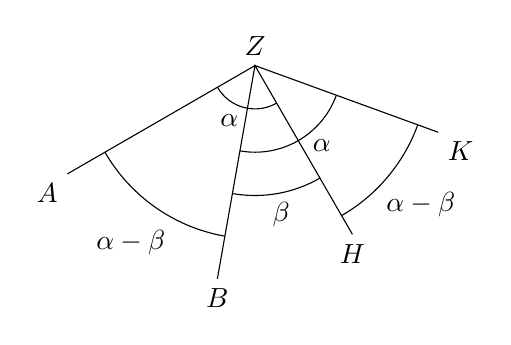
\begin{tikzpicture}[scale=.55]
\coordinate (Z) at (0,0);
\coordinate (A) at (-150:5cm);
\coordinate (B) at (-100:5cm);
\coordinate (H) at (-60:4.5cm);
\coordinate (K) at (-20:4.5cm);
\draw (A) node[below left] {$A$} -- (Z) node[above] {$Z$} -- (B) node[below] {$B$};
\draw (H) node[below] {$H$} -- (Z) -- (K) node[below right] {$K$};
\draw (-150:1cm) arc (-150:-60:1);
\draw (-100:2cm) arc (-100:-20:2);
\draw (-100:3cm) arc (-100:-60:3);
\draw (-150:4cm) arc (-150:-100:4);
\draw (-60:4cm) arc (-60:-20:4);
\node at (-115:1.4) {$\alpha$};
\node at (-50:2.4) {$\alpha$};
\node at (-80:3.5) {$\beta$};
\node at (-40:5) {$\alpha - \beta$};
\node at (-125:5) {$\alpha - \beta$};
\end{tikzpicture}
}
\end{center}
\leftcaption{Construction of  $x=\frac{n}{m}s$, step 3}\label{f.compass-relative3}
\rightcaption{$\angle AZB=\angle HZK$}\label{f.compass-relative4}
\end{figure}

$\triangle ZAB\sim\triangle ZHK$ since both are isosceles triangles and we have shown that they have the same vertex angle. Label $\overline{HK}$ by $x$. Then:
\begin{eqnarray*}
\frac{m}{s} &=& \frac{n}{x}\\
x&=&\frac{n}{m}s\,.
\end{eqnarray*}

\end{proof}


%%%%%%%%%%%%%%%%%%%%%%%%%%%%%%%%%%%%%%%%%%%%%%%%%%%%%%%%%%%%%%%

\section{Construction of the Intersection of Two Lines}\label{s.two-lines}

\begin{theorem}
Given two lines containing the line segments $\overline{AB}, \overline{CD}$, it is possible to construct their intersection $S$.
\end{theorem}

\begin{proof}
Let $C',D'$ be the reflections of $C,D$ around $\overline{AB}$.
There are two cases depending on whether $C,D$ lie on the same side of $\overline{AB}$ or on different sides. Label $x=\overline{CS}, c=\overline{CC'}, d=\overline{DD'}, e=\overline{CD}$ as shown in Figs.~\ref{f.compass-intersection1}, \ref{f.compass-intersection2}. We compute the value of $x$ for each case.

\textit{Case 1:}
$C,D$ are on the different sides of $\overline{AB}$.
$S$ lies on $\overline{AB}$ because $\triangle CZS\cong \triangle C'ZS$ by side-angle-side: $\overline{CZ}=\overline{C'Z}$, $\angle CZS=\angle C'ZS=90^\circ$ and $\overline{ZS}$ is a common side. Therefore $\overline{C'S}=\overline{CS}$ and similarly $\overline{D'S}=\overline{DS}$. $\triangle CSC'\sim\triangle DSD'$ are similar so $\displaystyle\frac{x}{e-x} = \displaystyle\frac{c}{d}$ and solving the equation gives $x=\displaystyle\frac{c}{c+d}e$.

\begin{figure}[ht]
\begin{center}
\begin{tikzpicture}[scale=.9]
\coordinate (A) at (-4,0);
\coordinate (B) at (2,0);
\coordinate (C) at (-3,2);
\coordinate (D) at (1,-1);
\coordinate (Cp) at (-3,-2);
\coordinate (Dp) at (1,1);
\vertex{A};
\vertex{B};
\node[below] at (A) {$A$};
\node[below] at (B) {$B$};
\node[above] at (C) {$C$};
\node[below] at (D) {$D$};
\node[below] at (Cp) {$C'$};
\node[above] at (Dp) {$D'$};
\draw[name path=ab] ($(A)!1.3!(B)$) -- ($(B)!1.3!(A)$);
\draw[name path=cd] ($(C)!1.2!(D)$) -- ($(D)!1.1!(C)$);
\path [name intersections={of=ab and cd,by={S}}];
\node[above] at (S) {$S$};
\draw (Cp) -- node[below] {$x$} (S);
\draw (S) -- node[above,xshift=-5pt] {$e\!-\!x$} (Dp);
\draw (C) -- node[above left,yshift=6pt] {$c$} (Cp);
\draw (D) -- node[above right,yshift=6pt] {$d$} (Dp);
\path (C) -- node[right,xshift=2pt] {$x$} (S);
\path (S) -- node[left,near end,xshift=-2pt] {$e\!-\!x$} (D);
\node[below left] at (C|-A) {$Z$};
\vertex{C};
\vertex{D};
\vertex{Cp};
\vertex{Dp};
\draw ($(C)!.5!(Cp)$) rectangle +(6pt,6pt);
\draw[rotate=90] ($(D)!.5!(Dp)$) rectangle +(6pt,6pt);
\end{tikzpicture}
\end{center}
\caption{Construction of  the intersection of two lines (1)}\label{f.compass-intersection1}
\end{figure}

\textit{Case 2:}
$C,D$ are on the same side of $\overline{AB}$. $\triangle CSC'\sim\triangle DSD'$ gives $\displaystyle\frac{x}{x-e}=\frac{c}{d}\displaystyle$ and solving the equation gives $x=\displaystyle\frac{c}{c-d}e$.

\begin{figure}[t]
\begin{center}
\begin{tikzpicture}[scale=.9]
\coordinate (A) at (-4,0);
\coordinate (B) at (2,0);
\coordinate (C) at (-3,2);
\coordinate (D) at (-1,1);
\coordinate (Cp) at (-3,-2);
\coordinate (Dp) at (-1,-1);
\vertex{A};
\vertex{B};
\node[below] at (A) {$A$};
\node[below] at (B) {$B$};
\node[above] at (C) {$C$};
\node[above] at (D) {$D$};
\node[below] at (Cp) {$C'$};
\node[below] at (Dp) {$D'$};
\draw[name path=ab] ($(A)!1.3!(B)$) -- ($(B)!1.3!(A)$);
\draw[name path=cd] ($(C)!2.2!(D)$) -- ($(D)!1.1!(C)$);
\path [name intersections={of=ab and cd,by={S}}];
\node[above] at (S) {$S$};
\draw (Cp) -- (S);
\draw (C) -- node[above left,yshift=6pt] {$c$} (Cp);
\draw (D) -- node[above right,yshift=6pt] {$d$} (Dp);
\path (C) -- node[above] {$e$} (D);
\path (Cp) -- node[below] {$e$} (Dp);
\path (D) -- node[above right,xshift=-4pt] {$x-e$} (S);
\path (Dp) -- node[below right,xshift=-4pt] {$x-e$} (S);
\node[below left] at (C|-A) {$Z$};
\vertex{C};
\vertex{D};
\vertex{Cp};
\vertex{Dp};
\draw ($(C)!.5!(Cp)$) rectangle +(6pt,6pt);
\draw[rotate=90] ($(D)!.5!(Dp)$) rectangle +(6pt,6pt);
\end{tikzpicture}
\end{center}
\caption{Construction of  the intersection of two lines (2)}\label{f.compass-intersection2}
\end{figure}

\medskip

Construct the circles $c(C',d), c(D,e)$ and denote their intersection by $H$ (Fig.~\ref{f.compass-intersection3}). The sum of the line segments $\overline{CC'}, \overline{C'H}$ is $c + d$. We have to show that $H$ is on the extension of $\overline{CC'}$ so that $\overline{CH}$ is a line segment of length $c+d$. $\overline{CH} = c - d$ in case $D$ is on the same side of $\overline{AB}$ as $C$ (not shown in the diagram).
\begin{figure}[b]
\begin{center}
\begin{tikzpicture}[scale=.8]
\coordinate (A) at (-4,0);
\coordinate (B) at (2,0);
\coordinate (C) at (-3,2);
\coordinate (D) at (1,-1);
\coordinate (Cp) at (-3,-2);
\coordinate (Dp) at (1,1);
\vertex{A};
\vertex{B};
\node[below left] at (A) {$A$};
\node[below] at (B) {$B$};
\node[above] at (C) {$C$};
\node[below] at (D) {$D$};
\node[left] at (Cp) {$C'$};
\node[above] at (Dp) {$D'$};
\draw[name path=ab] ($(A)!1.3!(B)$) -- ($(B)!1.3!(A)$);
\draw[name path=cd] ($(C)!1.2!(D)$) -- ($(D)!1.1!(C)$);
\path [name intersections={of=ab and cd,by={S}}];
\node[above,yshift=4pt] at (S) {$S$};
\draw (Cp) -- node[below right,xshift=5pt,yshift=5pt] {$e$} (Dp);
\path (C) -- node[above left] {$c$} (Cp);
\draw[thick,dashed] (D) -- node[above right] {$d$} (Dp);
\draw[name path=circled] (D) let
  \p1 = ($ (D) - (C) $),
  \n2 = {veclen(\x1,\y1)}
in
  ++(130:\n2) arc (130:230:\n2);

\draw[name path=circlecp] (Cp) let
  \p1 = ($ (D) - (Dp) $),
  \n2 = {veclen(\x1,\y1)}
in
  ++(-180:\n2) arc (-180:0:\n2);
\path [name intersections={of=circled and circlecp,by={H}}];
\node[below left] at (H) {$H$};
\draw ($(C)!1.2!(H)$) -- (C);
\draw (H) -- node[right] {$d$} (Cp);
\draw (D) -- node[right,xshift=18pt,yshift=12pt] {$e$} (H);
\vertex{Cp};
\vertex{D};
\vertex{C};
\vertex{Dp};
\vertex{H};
\path (C) -- node[above] {$x$} (S);
\path (Cp) -- node[below] {$x$} (S);
\end{tikzpicture}
\end{center}
\caption{Construction of  the intersection of two lines (3)}\label{f.compass-intersection3}
\end{figure}

$H$ is the intersection of $c(C',d), c(D,e)$ so $\overline{DH}=e$, $\overline{C'H}=d$. By construction $\overline{C'D'} = e$, $\overline{D'D}=d$ so the quadrilateral $\overline{C'D'DH}$ is a parallelogram. 

By construction $\overline{DD'}\parallel\overline{CC'}$ so $\overline{C'H}\parallel \overline{DD'}$ and therefore $\overline{C'H}\parallel\overline{CC'}$. Since one of its end points is $C'$ it must be on the line containing $\overline{CC'}$. By Thm.~\ref{thm.add-subtract-mm}, from the lengths $c,d,e$ a line segment of length $c+d$ can be constructed and by Thm.~\ref{thm.compass-ratio} a line segment of length $x=\displaystyle\frac{c}{c+d}e$ can be constructed. $S$, the intersection of $c(C',x)$ and $c(C,x)$, is also the intersection of $\overline{AB}, \overline{CD}$ (Fig.~\ref{f.compass-intersection4}).
\end{proof}

\begin{figure}[t]
\begin{center}
\begin{tikzpicture}[scale=.9]
\coordinate (A) at (-4,0);
\coordinate (B) at (2,0);
\coordinate (C) at (-3,2);
\coordinate (D) at (1,-1);
\coordinate (Cp) at (-3,-2);
\coordinate (Dp) at (1,1);
\vertex{A};
\vertex{B};
\node[below left] at (A) {$A$};
\node[below] at (B) {$B$};
\node[above] at (C) {$C$};
\node[below] at (D) {$D$};
\node[left] at (Cp) {$C'$};
\node[above] at (Dp) {$D'$};
\draw[name path=ab] ($(A)!1.3!(B)$) -- ($(B)!1.3!(A)$);
\draw[name path=cd] ($(C)!1.2!(D)$) -- ($(D)!1.1!(C)$);
\path [name intersections={of=ab and cd,by={S}}];
\node[above,yshift=4pt] at (S) {$S$};
\draw (Cp) -- (Dp);
\path (C) -- node[above,yshift=4pt] {$x$} (S);
\path (Cp) -- node[below,yshift=-4pt] {$x$} (S);
\path (C) -- node[above left] {$c$} (Cp);
\draw (D) -- node[above right] {$d$} (Dp);
\draw[name path=circled] (C) let
  \p1 = ($ (S) - (C) $),
  \n2 = {veclen(\x1,\y1)}
in
  ++(-10:\n2) arc (-10:-100:\n2);

\draw[name path=circlecp] (Cp) let
  \p1 = ($ (S) - (C) $),
  \n2 = {veclen(\x1,\y1)}
in
  ++(100:\n2) arc (100:0:\n2);
\draw (Cp) -- (C);
\vertex{C};
\vertex{Cp};
\vertex{D};
\vertex{Dp};
\end{tikzpicture}
\end{center}
\caption{Construction of  the intersection of two lines (4)}\label{f.compass-intersection4}
\end{figure}


%%%%%%%%%%%%%%%%%%%%%%%%%%%%%%%%%%%%%%%%%%%%%%%%%%%%%%%%%%%%%%%

\section{Construction of the Intersection of a Line and a Circle}\label{s.line-circle}

\begin{theorem}
Given a circle $k=C(M,r)$ and a line $l$ it is possible to construct the intersections of $k$ and $l$.
\end{theorem}

\begin{proof}
Construct $M'$, be the reflection of $M$ around $l$ and construct the circle $k'=c(M',r)$. Since $MYM'\cong\triangle MXM'$, $X,Y$, the points of intersection of $k,k'$, are the points of intersection of $l$ and $k$ (Fig.~\ref{f.compass-circle4}).
\begin{figure}[t]
\begin{center}
\begin{tikzpicture}[scale=.5]
\coordinate (A) at (-7,0);
\coordinate (B) at (8,0);
\coordinate (M) at (0,-2);
\coordinate (Mp) at (0,2);
\node[below left] at (M) {$M$};
\node[above left] at (Mp) {$M'$};
\draw[name path=c1] (M) circle[radius=3cm];
\draw[name path=c2] (Mp) circle[radius=3cm];
\draw[name path=ab] ($(A)!1.2!(B)$) --
  node[above,very near end] {$l$} ($(B)!1.2!(A)$);
\path [name intersections={of=c1 and c2,by={S1,S2}}];
\path[name path=radius1] (M) -- ++(15:4cm);
\path [name intersections={of=c1 and radius1,by={R1}}];
\draw (M) -- node[below] {$r$} (R1);
\path[name path=radius2] (Mp) -- ++(40:4cm);
\path [name intersections={of=c2 and radius2,by={R2}}];
\draw (Mp) -- node[above] {$r$} (R2);
\draw (Mp) -- (M) -- (S1) -- (Mp) -- (S2) -- (M);
\node[right,xshift=6pt,yshift=6pt] at (S1) {$X$};
\node[left,xshift=-6pt,yshift=6pt] at (S2) {$Y$};
\draw (0,0) rectangle +(10pt,10pt);
\node at (-3.5,-3) {$k$};
\node at (-3.5,3) {$k'$};
\end{tikzpicture}
\end{center}
\caption{Construction of  the intersection of a line and a circle (1)}\label{f.compass-circle4}
\end{figure}

This construction cannot be done if $M$ is on the line $l$. In that case choose an arbitrary point $A$ on $l$ that is at a distance more than $r$ from $M$. Using Thm~\ref{thm.add-subtract-mm} shorten and lengthen $\overline{AM}$ by $r$. $X,Y$, the endpoints of these segments, are the intersections of $k$ and $l$ (Fig.~\ref{f.compass-circle5}).
\end{proof}

\begin{figure}[b]
\begin{center}
\begin{tikzpicture}[scale=.5]
\coordinate (A) at (-7,0);
\coordinate (B) at (8,0);
\coordinate (M) at (0,0);
\vertex{M};
\vertex{A};
\node[below] at (A) {$A$};
\node[below left] at (M) {$M$};
\draw[name path=c1] (M) circle[radius=3cm];
\draw[name path=ab] ($(A)!1.2!(B)$) -- 
  node[above,very near end] {$l$} ($(B)!1.2!(A)$);
\path[name path=radius1] (M) -- ++(50:4cm);
\path [name intersections={of=c1 and radius1,by={R1}}];
\draw (M) -- node[above] {$r$} (R1);
\path [name intersections={of=c1 and ab,by={S1,S2}}];
\node[above right] at (S1) {$X$};
\node[above left] at (S2) {$Y$};
\path (M) -- node[below,xshift=4pt] {$\overline{AM}+r$} (S1);
\path (A) -- node[below] {$\overline{AM}-r$} (S2);
\node at (-2.5,2.5) {$k$};
\end{tikzpicture}
\end{center}
\caption{Construction of  the intersection of a line and a circle (2)}\label{f.compass-circle5}
\end{figure}
\index{Construction!compass@with only a compass|)}

\newpage

\subsection*{What Is the Surprise?}

When one learns about constructions with a straightedge and compass it is obvious that both tools are necessary. Therefore,  it was quite a surprise to find out that a compass is sufficient. The proof is quite long so we are not going to leave the straightedge at home, but the theorem shows that we should not assume that there are no alternatives to well-known mathematical concepts.

\subsection*{Sources}

This chapter is based on problem $33$ of \cite{dorrie1} reworked by Michael Woltermann \cite{dorrie2}. An additional proof can be found in \cite{mm}.
